\section{Materiales y métodos}

Se ha llevado a cabo un estudio fenotípico sobre la población afectada por el fenómeno de Raynaud. Se pretende averiguar la influencia de los diferentes genes asociados a la enfermedad y su grado de importancia en el desarrollo de la misma.

Para llevar acabo la siguiente metodología hemos será necesario descargar la última versión de R, que, hasta la fecha de este proyecto es la 4.2.1 . Así como será necesario instalar todas las librerías indicadas en el repositorio de github.

\begin{figure}
	\centering
	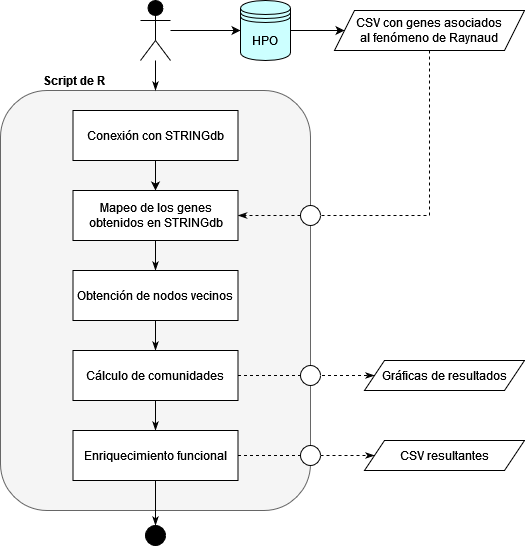
\includegraphics[width=0.4\textwidth]{figures/Workflow_genes.PNG}
	\caption{Flujo de Trabajo}
	\label{workflow}
\end{figure}

\subsection{Obtención de la red}
\label{obtencion_red}
STRINGdb es una base de datos open-source que busca integrar todas las relaciones conocidas entre proteínas, así como sus interacciones físicas o funcionales. Esta herramienta también nos permite visualizar las redes que forman un conjunto de proteínas. Para la obtención automática de los datos es necesario utilizar la API de STRINGdb con R. Al tratarse de un estudio sobre una enfermedad que afecta a humanos, es necesario descargar de 'string' todas las proteínas, interacciones y peso de el enlace; del genoma humano al completo. El ID taxonómico con el que realizar la búsqueda es el \textbf{9606}. Como ya se ha comentado en el apartado \ref{genes_asociados} y como podemos ver en \ref{fig:workflow} es necesario descargar de HPO el nombre de los genes asociados, su rentrez\_ID (que será útil para el mapeo de nuestros genes en el genoma) y el identificador del gen de la base de datos de OMIM; Todos estos datos relacionados con el fenómeno de Raynaud. Finalmente mediante haciendo uso de la API de STRINGdb realizamos un mapeo de los identificadores de rentrez de nuestros genes con la red completa del genoma humano de STRINGdb. Obteniendo así los genes con los que realizaremos el estudio.

\subsection{Cálculo de comunidades}

Tras conseguir los datos ahora debemos de realizar un estudio del grafo obtenido a partir de los datos del apartado \ref{obtencion_red}.Para ellos realizamos un subgrafo a partir del mapeo de genes del apartado anterior para guardar nuestros datos en un objeto de tipo grafo. Como ya sabemos un grafo es un conjunto de nodos unidos por enlaces llamados aristas que nos permite representar las relaciones entre elementos de un conjunto. Haciendo uso de la teoría de grafos sabiendo que la vecindad de un vértice en un grafo G es el subgrafo inducido de G que está formado por todos los vértices adyacentes y todas las aristas que conecten dichos nodos. En otras palabras aplicado a nuestros datos, vamos a obtener aquellos nodos que presenten un mayor número de relaciones para dividir todos nuestros genes en diferentes clusters. Cada cluster obtenido es una comunidad diferente, las ventajas que nos proporciona esto es el poder estudiar cada una por separado y realizar análisis de expresión solo a aquellos genes coexpresados. \cite{} \cite{}

\subsection{Enriquecimiento funcional}

El análisis de enriquecimiento de conjuntos (\textit{Gene Sequence Enrinchment Analysis} \ref{GSEA}) es un método para identificar clases de genes o proteínas que están sobrerepresentadas o empobrecidas en una comunidad de genes y pueden tener asociación con fenotipos de enfermedades. Los métodos de GSEA se basan en métodos estadísticos y en las últimas tecnologías de transcriptómica y proteómica.

\subsubsection{GO}
La base de datos de GO \ref{GO}. Al realizar un enriquecimiento mediante GO conseguimos en formato tabla los términos GO compartidos significativos con los genes a los que aplicamos el enriquecimiento, así como su valor de sobrerrepresentación / subrepresentación y su valor p asociado. El valor p es l probabilidad de ver al menos \textit{x} número de genes del total de genes en la lista anotados a un término GO en particular, dada la proporción de genes en todo el genoma. \\

\subsubsection{KEGG}
La base de datos de KEGG (\textit{Kyoto Encyclopedia of Genes and Genomes} \ref{KEGG}). KEGG es una base de datos que integra información genómica, química y de funciones del sistema. El núcleo de estos son las bases de datos KEGG pathway y KEGG orthology. En la base de datos KEGG pathway, las vías metabólicas biológicas se dividen en 6 categorías: procesos celulares, procesamiento de información ambiental, procesamiento de información genética, enfermedades humanas, metabolismo y sistemas orgánicos. \\

Tras aplicar sendos enriquecimientos para cada comunidad que obtenemos en nuestro script de R. Obtenemos datos tabulador que nos serán útiles para realizar un estudio de funcionalidad de cada comunidad y sacar las conclusiones pertinentes.